\chapter{Background Theory}
%OR: \chapter{Tools and Methods}
\label{cha:background-theory}

\begin{comment}
The background theory depth and breadth depend on the depth needed to understand your project
in the different disciplines that your project crosses.
It is not a place to just write about everything you know that is vaguely connected to your project.
The theory is here to help the readers that do not know the theoretical basis of your work so that they
can gain sufficient understanding to understand your contributions --- and also for yourself to show that
you have understood the underlying theory and are aware of the methods used in the field.
In particular, the theory section provides
an opportunity to introduce terminology that can later be used without disturbing the text with a definition.
In some cases it will be more appropriate to have a separate section for different theories (or even separate chapters).
However, be careful so that you do not end up with too short sections.
Subsections may also be used to separate different background theories.

Be aware that ``background'' is a general term that refers to everything done by somebody else,
in contrast to the ``foreground'', which is your own work.
Hence there can (and will) be several background chapters, with the background theory being one of them
--- or several of them, since it thus is quite possible to split the background theory over more than one chapter,
e.g., by having a chapter introducing the theory directly needed for the research field in question and another
chapter discussing the machine learning theory, algorithms, tools, and evaluation methods commonly used in the field.
The related work chapter is thus also part of the background, while a chapter about data might be background
(if you only use somebody else datasets), but can also be part of the foreground (if you collect and/or annotate data
yourself, or if you process or clean the data in ways that can make it part of your own contribution).

It is ok to reuse material from other texts that you have written (e.g., the specialisation project), but if you do so, that must be clearly stated in the text, together with a description of how much of the text is new, old or rewritten/edited.
Such a statement about recycling of material in the Background Theory chapter can thus come here in the chapter introduction.

\section{Writing References in the Text}
\label{sec:writing_references}

When introducing techniques or results, always reference the source.
Be careful to reference the original contributor of a technique and not just someone who happens to use the technique.%
\footnote{But always make sure that you have read the work you are citing --- if not, cite someone who has!}
For results relevant to your work,
you would want to look particularly at newer results so that you have referenced the most up-to-date work in your area.
A common rule of thumb is to at least reference the first paper introducing the issue and the paper containing the latest / state-of-the-art
results. Additional papers making substantial contributions should also be referenced, as well as of course the ones you find most interesting.
Remember to use the right verb form depending on the number of authors.

If you do not have the source handy when writing, mark in the text that a reference is needed and add it later. \todo{add reference}
Web pages are not reliable sources --- they might be there one day and removed the next; and thus should be avoided, if possible.
A verbal discussion is not a source and should normally not be referenced
(though you can reference ``personal communication'', if there are no other options).
The bulk of citations in the report will appear in Chapter~\ref{cha:related_work}.
However, you will often need to introduce some terminology and key citations already in this chapter.

You can cite a paper in the following manner (and several other versions,
see the \verb!natbib! package documentation):

\begin{enumerate}[(i)]
    \item When referring to authors, using their names in the text:\\
          \citet{Authorson;Bobsen:10} stated something rather nice.
          (using \verb!\citet!)
    \item To cite indirectly: \\
          Papers should be written nicely \citep{Authorson;Bobsen:10}
          (using \verb!\citep!)
          {\em or\/}\\
          In \citet{Authorson;Bobsen:10}, a less detailed template was presented.
    \item To just cite the authors: \\
          \citeauthor{Authorson;Bobsen:10} wrote a nice paper
          (using \verb!\citeauthor!).
    \item Or just the year: \\ \citeyear{Authorson;Bobsen:10}
          (using \verb!\citeyear!).
    \item You can even cite specific pages or chapters: \citet[p. 3]{Authorson;Bobsen:10}
          (using \verb!\citet[...]{...}!).
\end{enumerate}

You should obviously always cite your supervisor's work \citep{BenyonEA:13},
even if it is completely irrelevant \citep{Das;Gamback:13a} or very old \citep{AlshawiEA:91b}.
Digging up an even older book can also appear impressive \citep{Diderichsen:57}.
(Or? ;-)

\section{The Reference List}
\label{sec:reference_list}

In general, make sure that the references that appear in your reference list can be easily located and identified by the reader.
So include not only authors and title, but year and place of publication, the full names of conferences and workshops,
page numbers in proceedings and collections, etc.
Hyperlinks or \acrfull{acr:doi} numbers are also nice to include.
Just as in the text itself, it is important to be consistent in the reference list, so include the same type of information for all references and write it in the same way.

Check out the reference list at the end of this document for examples of how to write references in \BibTeX.
Note a particular quirk: Many \BibTeX\ styles convert uppercase letters to lowercase, unless specifically told not to.
You might thus need to ``protect'' characters that should not be converted, e.g., by writing \texttt{\{T\}witter} as in the \citet{FountaEA:18} reference.

Also, keep in mind that `et' is a word in its own right (`and'), so there is no period after it (even though there is a period after `al.', which is short for `alia', meaning `others').
Of course, when including such a reference in the text, the authors should be referred to in plural form.
So \citet{BenyonEA:13} state that life is good (not ``states'').

Many sites, such as journals and \url{dblp.org} provide the matching \BibTeX\ entry for a reference.
However, you might still need to edit the entry in order to be consistent with the rest of your references.
If you find references from sites such as \url{scholar.google.com} or \url{arXiv.org}, keep in mind that they often not are complete,
so that you might need to add information to the entry (and probably edit it as well).

Some other good sites to find state-of-the-art work:
\begin{itemize}
    \item \url{paperswithcode.com}
    \item \url{nlpprogress.com}

\end{itemize}

\textit{Lorem ipsum dolor sit amet, consectetur adipiscing elit, sed do eiusmod tempor incididunt ut labore et dolore magna aliqua. Ut enim ad minim veniam, quis nostrud exercitation ullamco laboris nisi ut aliquip ex ea commodo consequat. Duis aute irure dolor in reprehenderit in voluptate velit esse cillum dolore eu fugiat nulla pariatur. Excepteur sint occaecat cupidatat non proident, sunt in culpa qui officia deserunt mollit anim id est laborum.}

\begin{figure}[t!]
    \centering
    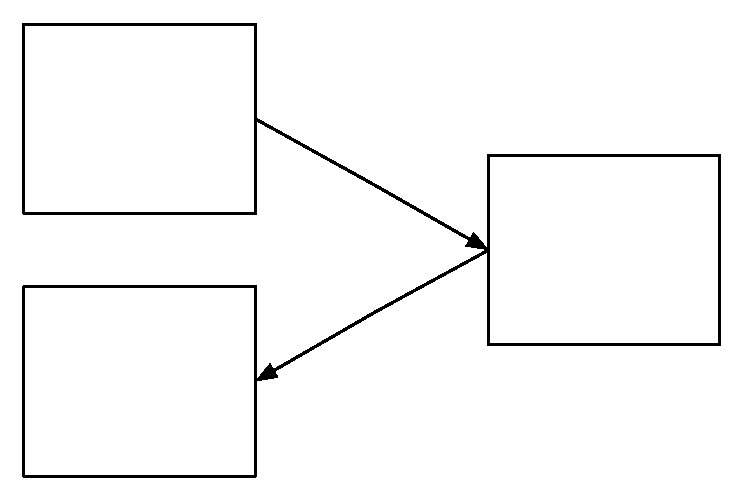
\includegraphics[width=0.5\columnwidth]{figs/figure1.pdf}
    \caption[Boxes and arrows are nice]{Boxes and arrows are nice (adapted from \citealp{Authorson;Bobsen:10}, reprinted with permission)}
    \label{fig:BoxesAndArrowsAreNice}
\end{figure}

\section{Introducing Figures}

\LaTeX is a bit tricky when it comes to the placement of ``flooting bodies'' such as figures and tables. It is often a good idea to let their code appear right before the header of the (sub)section in which they appear.
Note that you should anyhow always use an option for the placement (e.g., \verb|[t!]| to place it at the top of a page).

Remember that if you reproduce someone else's figures you must credit the original author --- such as
Figure~\ref{fig:BoxesAndArrowsAreNice} (adapted from \citealp{Authorson;Bobsen:10}),
as well as state that you have permission to reprint it (e.g., if it is published under a Creative Commons License,
or if you have gained explicit permission from the author).

Do not just put the figure in and leave it to the reader to try to understand what the figure is.
The figure should be included to convey a message and you need to help the reader to understand the message
intended by explaining the figure in the text.
Hence \textbf{all} figures and tables should always be referenced in the text, using the \verb!\ref! command.
It is good practice to always combine it with a non-breakable space (\verb!~!) so that there will be no newline between the term referring to it and the reference, that is, using \verb!Figure~\ref{fig:BoxesAndArrowsAreNice}!.

If a figure appears far from the text explaining it,
it is a good idea to add its page number (using the \verb!\pageref! command), so that you can refer to Figure~\ref{fig:BoxesAndArrowsAreNice} (on Page~\pageref{fig:BoxesAndArrowsAreNice}).

Also, note that you can have a longer version of the figure (and table) caption attached to the actual figure,
while using the optional first argument to \verb!\caption! to include a shorter version in the list of figures (lof) or list of tables:
\begin{quote}
    \begin{verbatim}
\caption[Shorter lof text]{Longer text appearing under the figure}
\end{verbatim}
\end{quote}

It is good practice to add a note about a missing figure in the text,
such as the completely amazing stuff that will appear in Figure~\ref{fig:AmazingFigure}.

\begin{figure}[t!]
    \centering
    \missingfigure{Here we will add an amazing figure explaining it all}
    \caption{A missing figure}
    \label{fig:AmazingFigure}
\end{figure}

In general it is good to add notes about things that you plan on writing later.
The \verb!todonotes! package is great for that kind of book-keeping, letting you write both shorter comments in the margin\todo{l8r dude} and longer comments inside the text, using the option \verb![inline]!.
\todo[inline]{There are always some more stuff that you will need to add at some later point.
    Be sure to at least make a note about it somewhere.}

\textit{Sed ut perspiciatis unde omnis iste natus error sit voluptatem accusantium doloremque laudantium, totam rem aperiam, eaque ipsa quae ab illo inventore veritatis et quasi architecto beatae vitae dicta sunt explicabo. Nemo enim ipsam voluptatem quia voluptas sit aspernatur aut odit aut fugit, sed quia consequuntur magni dolores eos qui ratione voluptatem sequi nesciunt. Neque porro quisquam est, qui dolorem ipsum quia dolor sit amet, consectetur, adipisci velit, sed quia non numquam eius modi tempora incidunt ut.}

\section{Introducing Tables in the Report}

\newcommand\emc{-~~~~}
\begin{table}[t!]
    \centering
    \caption[Example table]{Example table (F$_1$-scores); this table uses the optional shorter caption that will appear in the list of tables, so this long explanatory text will not appear in the list of tables and is only here in order to explain that to the reader.}
    \begin{tabular}{c|c|rrrrrr}
        \tabletop
        Langs                  & Source                                           & \multicolumn{1}{c}{Lang1} & \multicolumn{1}{c}{Lang2} & \multicolumn{1}{c}{Univ} & \multicolumn{1}{c}{NE} & \multicolumn{1}{c}{Mixed} & \multicolumn{1}{c}{Undef}
        \\ \tablemid
        \multirow{5}{*}{EN-HI} & FB+TW                                            & 54.22                     & 22.00                     & 19.70                    & 4.00                   & 0.05                      & 0.03                      \\
                               & FB                                               & 75.61                     & 4.17                      & 18.00                    & 2.19                   & 0.02                      & 0.01                      \\
                               & TW                                               & 22.24                     & 48.48                     & 22.42                    & 6.71                   & 0.08                      & 0.07                      \\
                               & Vyas                                             & 54.67                     & 45.27                     & 0.06                     & \emc                   & \emc                      & \emc                      \\
                               & FIRE                                             & 45.57                     & 39.87                     & 14.52                    & \emc                   & 0.04                      & \emc                      \\ \tablemid
        \multirow{2}{*}{EN-BN} & TW                                               & 55.00                     & 23.60                     & 19.04                    & 2.36                   & \emc                      & \emc                      \\
                               & FIRE                                             & 32.47                     & 67.53                     & \emc                     & \emc                   & \emc                      & \emc                      \\ \tablemid
        EN-GU                  & FIRE                                             & 5.01                      & \textbf{94.99}            & \emc                     & \emc                   & \emc                      & \emc                      \\
        \tablemid
        DU-TR                  & Nguyen                                           & 41.50                     & 36.98                     & 21.52                    & \emc                   & \emc                      & \emc                      \\ \tablemid

        EN-ES                  & \multirow{4}{*}{\rotatebox[origin=c]{90}{EMNLP}}
                               & 54.79                                            & 23.50                     & 19.35                     & 2.08                     & 0.04                   & 0.24                                                  \\
        EN-ZH                  &                                                  & 69.50                     & 13.95                     & 5.88                     & 10.60                  & 0.07                      & \emc                      \\
        EN-NE                  &                                                  & 31.14                     & 41.56                     & 24.41                    & 2.73                   & 0.08                      & 0.08                      \\
        AR-AR                  &                                                  & 66.32                     & 13.65                     & 7.29                     & 11.83                  & 0.01                      & 0.90                      \\ \tablebot
    \end{tabular}
    \label{tab:ExampleTable}
\end{table}

As you can see from Table~\ref{tab:ExampleTable}, tables are nice.
However, again, you need to discuss the contents of the table in the text.
You do not need to describe every entry, but draw the reader's attention to what is important in the table,
e.g., that 94.99 is an amazing F$_1$-score (and that probably something fishy happened there).
Use boldface, boxes, colours, arrows, etc. to mark the important parts of the table.

As can be seen in the example, elements in a table can sometimes benefit from being rotated (such as EMNLP in the `Source' column) or cover more than one row (EMNLP, as well as EN-HI and EN-BN in the `Langs' column) --- or more than one column, for that matter.

\textit{Donec non turpis nec neque egestas faucibus nec id neque. Etiam consectetur, odio vitae gravida tempus, diam velit sagittis turpis, a molestie ligula tellus at nunc. Proin dolor neque, dapibus a pellentesque a, commodo a nibh.}
\end{comment}

\Autochapterref{cha:background-theory} will lay a theoretical basis for the work done in this master thesis, providing the user with the required understanding in order to understand the contributions of the work. \Autosectionref{sec:language-modelling} will explain the theoretical basis of the component which most modern \glspl{acr:llm} are based upon --- namely the Transformer --- and the attention mechanism within it. The section will also touch upon a new approach to language modelling called \textit{selective state space modelling}, which has yielded very promising results for small \glspl{acr:llm}.

\vspace{12pt}

\begin{itshape}
    \noindent Parts of the Background chapter is reused material from the specialization project \citep{holmLLMsDeathGIS2023} preceding this master thesis. Below are the sections in question, together with a description of the extent to which, and how, the material is reused:

    \begin{itemize}
        \item \Autosubsectionref{subsec:attention-and-the-transformer-architecture}: Reused without modification.
        \item \Autosubsectionref{subsec:the-gpt-family}: Reused without modification.
    \end{itemize}
\end{itshape}


\section{Approaches to Language Modelling}
\label{sec:language-modelling}

\Autosubsectionref{subsec:attention-and-the-transformer-architecture} will explain the theoretical basis behind most modern \glspl{acr:llm}, which are based upon the attention mechanism built into the Transformer architecture. \Autosubsectionref{subsec:state-space-models} will explain modern state space-modelling approaches and why they may have a potential greater than Transformer-based models. First, however, \autoref{subsec:statistical-models-and-rnns} will delve into earlier attempts at language modelling.

\subsection[Early Attempts: Statistical Models and Recurrent Neural Networks]{Early Attempts: Statistical Models and \acrlongpl{acr:rnn}}
\label{subsec:statistical-models-and-rnns}

\subsection{Statistical Models}


\subsection[Recurrent Neural Networks]{\acrlongpl{acr:rnn}}


\subsection{Attention and the Transformer Architecture}
\label{subsec:attention-and-the-transformer-architecture}


\cite{vaswaniAttentionAllYou2017} managed to achieve new state-of-the-art results for machine translation tasks with their introduction of the Transformer architecture. The Transformer has later been proved effective for numerous downstream tasks, and for a variety of modalities. Titling their paper \citetitle{vaswaniAttentionAllYou2017}, \citeauthor{vaswaniAttentionAllYou2017} suggest that their attention-based architecture renders network architectures like \glspl{acr:rnn} redundant, due to its superior parallelization abilities and the shorter path between combinations of position input and output sequences, making it easier to learn long-range dependencies \citep[6]{vaswaniAttentionAllYou2017}.

The Transformer employs self-attention, which enables the model to draw connections between arbitrary parts of a given sequence, bypassing the long-range dependency issue commonly found with \glspl{acr:rnn}. An attention function maps a query and a set of key-value pairs to an output, calculating the compatibility between a query and a corresponding key \citep[3]{vaswaniAttentionAllYou2017}. Looking at \citeauthor{vaswaniAttentionAllYou2017}'s proposed attention function \eqref{eq:attention}, we observe that it takes the dot product between the query $Q$ and the keys $K$, where $Q$ is the token that we want to compare all the keys to. Keys similar to $Q$ will get a higher score, i.e., be \textit{more attended to}. These differences in attention are further emphasized by applying the softmax function. The final matrix multiplication with the values $V$ (the initial embeddings of the input tokens) will yield a new embedding in which all individual tokens have some context from all other tokens. We improve the attention mechanism by multiplying queries, keys, and values with weight matrices that are learned through backpropagation. Self-attention is a special kind of attention in which queries, keys, and values are all the same sequence.

\begin{equation}
    \text{Attention}(Q, K, V) = \text{softmax}\left(\frac{QK^T}{\sqrt{d_k}}\right)V
    \label{eq:attention}
\end{equation}

Attention blocks can be found in three places in the Transformer architecture \citep[5]{vaswaniAttentionAllYou2017} (I will use machine translation from Norwegian to German as an example):

\begin{enumerate}
    \item In the encoder block to perform self-attention on the input sequence (which is in Norwegian)
    \item In the decoder block to perform self-attention on the output sequence (which is in German)
    \item In the decoder block to perform cross-attention (also known as encoder-decoder attention) where each position in the decoder attends to all positions in the encoder
\end{enumerate}

The Transformer represented a breakthrough in the field of \gls{acr:nlp}, and is the fundamental building block of modern \glspl{acr:llm}, most famous of which are the \acrshort{acr:gpt}'s.

\subsection{State Space Models}
\label{subsec:state-space-models}

\section[State-of-the-Art Large Language Models]{State-of-the-Art \acrlongpl{acr:llm}}

\subsection{The GPT Family}
\label{subsec:the-gpt-family}

\gls{acr:gpt} is a type of \gls{acr:llm} that was introduced by OpenAI in 2018 \citep{radfordImprovingLanguageUnderstanding2018}. Specifically designed for text generation, a \acrshort{acr:gpt} is essentially a stack of Transformer \textit{decoders}. It demonstrates through its vast pre-training on unlabelled data that such unsupervised training can help a language model learn good representations, providing a significant performance boost while alleviating the dependence on supervised learning. While the original Transformer architecture as described by \cite{vaswaniAttentionAllYou2017} was intended for machine translation---thus having encoders to learn the representation of the origin language representation of a given input sequence and decoders to learn the representation in the target language and perform cross-attention between the two---the \acrshort{acr:gpt} is designed only to \textit{imitate} language. This is why there are no encoders to be found in the \acrshort{acr:gpt} architecture, only decoders. The model employs masked multi-head attention (running the input sequence through multiple attention heads in parallel), and is restricted to only see the last $k$ tokens---with $k$ being the size of the context window---and tasked to predict the next one.

Training consists of two stages: unsupervised pre-training and supervised fine-tuning. The former is used to find a good initialization point, essentially teaching the model to imitate the corpora upon which it is trained. This results in a model that will ramble on uncontrollably, just trying to elaborate upon the input sequence it's given to the best of its knowledge. This will naturally produce undefined behaviour, and it is therefore necessary to fine-tune the model on target tasks in a supervised manner. \cite[4]{radfordImprovingLanguageUnderstanding2018} explain how the model can be fine-tuned directly on tasks like text classification, but how one for other tasks needs to convert structured inputs into ordered sequences because the pre-trained model was trained on contiguous sequences of text. In the case of ChatGPT, \citeauthor{openaiIntroducingChatGPT2022} used \gls{acr:rlhf} by employing a three-step strategy: first training using a supervised policy, then using trained reward models to rank alternative completions produced by ChatGPT models, before fine-tuning the model using \gls{acr:ppo}, which is a way of training \acrshort{acr:ai} policies. This pipeline is then performed for several iterations until the model produces the desired behaviour \citep{openaiIntroducingChatGPT2022}.

\subsection{The Gemini  Family}
\subsection{The Claude Family}
\subsection{Open-Source Alternatives and Honourable Mentions}


\section[Function Calling LLMs]{Function Calling \acrshortpl{acr:llm}}
\label{sec:function-calling}

\textit{Function calling}---first introduced by OpenAI \citep{eletiFunctionCallingOther2023}---allows developers to provide function definitions to an \gls{acr:llm} and have said \gls{acr:llm} output a \acrshort{acr:json} object containing the name of one or more of the functions provided, as well as suitable arguments to these. Made possible through fine-tuning models to detect when functions should be calling, function calling makes it possible to give an \gls{acr:llm} \textit{hooks} into the real world, and provides a more reliable way for developers to integrate \glspl{acr:llm} into applications.

Possible use cases include using functions provide correct and up-to-date information that would otherwise require extensive training and fine-tuning. Having the \gls{acr:llm} use function calling for information retrieval also make them more transparent, making it possible to trace a claim back to its source, something that is normally a difficult feat with \gls{acr:llm}. Another use case might be code execution. One could imagine a rather simple function \texttt{execute\_python\_code(code: string) -> string} that takes Python code as a string and returns the standard output that results from executing that code. This is likely the principle behind products like OpenAI's Data Analysis mode (previously Code Interpreter), in which ChatGPT functions as a code executing agent that can generate, execute, and self-correct its own code. Similar functions could be constructed for \acrshort{acr:sql}, making it possible for \glspl{acr:llm} to work against relational databases. As \cite{eletiFunctionCallingOther2023} describes, function calling can also be used to extract structured data from text.




\glsresetall
